\documentclass[a4paper,12pt]{report}
\usepackage[margin=2cm]{geometry}
\usepackage[utf8]{inputenc}
\usepackage{listings} 
\usepackage{color}
\usepackage{xcolor}
\usepackage{hyperref}
%\usepackage{zeta}
%\usepackage[inline]{trackchanges}
\usepackage{pgf,pgfarrows,pgfnodes,pgfautomata,pgfheaps}
%\usepackage{makeidx}
\usepackage{tocloft}
%\usepackage{romanian}
\usepackage{pdfpages}

\definecolor{codegreen}{rgb}{0,0.6,0}
\definecolor{codegray}{rgb}{0.5,0.5,0.5}
\definecolor{codepurple}{rgb}{0.58,0,0.82}
\definecolor{backcolour}{rgb}{0.95,0.95,0.92}

\lstdefinestyle{mystyle}{
    backgroundcolor=\color{backcolour},   
    commentstyle=\color{codegreen},
    keywordstyle=\color{magenta},
    numberstyle=\tiny\color{codegray},
    stringstyle=\color{codepurple},
    basicstyle=\ttfamily\footnotesize,
    breakatwhitespace=false,         
    breaklines=true,                 
    captionpos=b,                    
    keepspaces=true,                 
    numbers=left,                    
    numbersep=5pt,                  
    showspaces=false,                
    showstringspaces=false,
    showtabs=false,                  
    tabsize=2
}

\begin{document}
\newcommand{\h}{\texttt}

\vspace{-5cm}
\begin{center}
Deitemment of Computer Science\\
Technical University of Cluj-Napoca\\
\pgfimage[width=15cm]{footer.jpg}
\end{center}
\vspace{1cm}
%\maketitle
\begin{center}
\begin{Large}
Knowledge-Based Systems\\
\end{Large}

\vspace*{1cm}
Laboratory activity 2021\\

\vspace*{1cm}
Car Configurator Ontology \\
\vspace*{1cm}

Team name: NoName\\
Students: Dragoteanu Bogdan, Rusu Andrei\\

\vspace*{14cm}

Assoc. Prof.dr. eng. Adrian Groza\\
Adrian.Groza@cs.utcluj.ro
\end{center}

\newpage 
\tableofcontents

\chapter{Competency questions and use cases}
\section{Competency questions}

\begin{itemize}
  \item Is item X compatible with model Y?
  \item Is item X compatible only with model Y?
  \item What models are compatible with item X?
  \item Is item X$_1$ compatible with item X$_2$?
  \item Is item X standard or optional?
  \item Is model Y an electric vehicle?
  \item What interior trim options are there for model Y?
  \item Does item X$_1$ include item X$_2$?
  \item Is item X an interior or exterior item?
  \item Is model Y available with large wheels?
  \item Is a glass roof available for model Y?
\end{itemize}

\section{Use Cases}
The main use cases are:
\begin{itemize}
  \item Finding out which configuration items are compatible with the desired vehicle
  \item Checking the compatibility of the items between themselves
  \end{itemize}

\chapter{Concepts}
The Car Configuration ontology is used for configuring a vehicle with the desired options.
Therefore, the options have to be divide into categories, and rules established for selecting items from them, so as to fit together.
Below is the preliminary classification of car configuration items:

\begin{center}
    \pgfimage[width=10cm]{car_config_ontology.png}
\end{center}

We have split the vehicles into two categories: electric and with combustion engines. The optional items are then split into Exterior and Interior items, where you would find your usual expected items.
Using this classification, we will be able to defines rules that specify that you may only choose one item from Wheels, but more then one item from Tech, for example.

Below is an extract from the Taxonomy page of Racer:

\begin{center}
    \pgfimage[width=15cm]{taxonomy.png}
\end{center}

\chapter{ABox}
We will briefly show the structure and knowledge present in the knowledge base

\chapter{Roles}
The roles we have defined are the following:
\begin{itemize}
    \item isCompatibleCarItem
    \item isCompatibleItemItem
    \item isIncluded
    
\end{itemize}

The role \textit{isCompatibleCarItem} defines which equipment items are compatible with a specified model, while the role \textit{isCompatibleItemItem} defines which items are compatible between each other. For example, two different sets of wheels are incompatible, since only one type of wheel can be selected in a car configuration.

\bigskip
The role \textit{isIncluded} specifies which items are included in other items, for example, the blind spot monitoring system is included in the full autopilot system.

\bigskip
Additionally, we have defined two additional attributes for each equipment item: \textit{price} and \textit{optional}, which show the price of an item and whether it is given as standard or it is an option. Standard equipment costs nothing.

\bigskip
Below is the formal declaration of the roles from above:
\bigskip

\textit{(define-primitive-role isCompatibleCarItem :domain CarType :range Item)}

\textit{(define-primitive-role isCompatibleItemItem :domain Item :range Item  :symmetric t)}

\textit{(define-primitive-role isIncluded :domain Item :range Item :asymmetric t)}

\chapter{Rules}
We have defined a rule that propagates the compatibility of a items to a vehicle model, when an item includes another item:

\begin{center}
    \textit{(define-rule (?car ?item2 isCompatibleCarItem)}
    
    \textit{(and (?car CarType) (?item1 Item) (?item2 Item) (not (same-as ?item1 ?item2))}
    
    \textit{(?car ?item1 isCompatibleCarItem) (?item2 ?item1 isIncluded))) }

\end{center} 

Meaning that vehicle ?car and item ?item2 are deemed compatible if there is another item ?item1 with which ?car is compatible and which also includes ?item2.

\bigskip
For example, if a vehicle is compatible with the FullAutopilot item, which includes the BlindSpotMonitor item, it then means that the vehicle is also compatible with the BlindSpotMonitor, however not at the same time.

\bigskip
In order to infer which items are compatible with other items, we decided to use the Racer Java API, since defining a set of rules that would produce this result in racer syntax proved too difficult.

We defined two items that are compatible as being from different sets. For example, a glass roof is compatible with 19' wheels, since they do not interfere with each other. However, 19; wheels are not compatible with 20' wheels, since a vehicle can only have one type of item from the Wheels category. Code is included in later chapters.  

\bigskip
It is also possible to count the instances of a set and, for example, say that only one item of some categories can be selected, but more from another category, like Safety for example. However, we removed the need for this extra verification by combining the items in item packs, that are like upgrades, with each pack containing the features of the previous pack, plus additional ones.

\bigskip
For example, the item HeatedSeats includes the item RegularSeats, which are both in the Seats category, meaning that only one can be selected as a configuration. The same goes for the FullAutopilot item, which includes the BlindSpotMonitor item and are both part of the Safety category. This way we can ensure that only one item from each category is selected.

\bigskip
Additionally, we have defined an extra rule that is applied between items with inclusions. It implements the transitivity property of the inclusion of items, which could not be defined in the rule definition of the \textit{isIncluded} role, due to the fact that inclusion is assimetrical:

\begin{center}

    \textit{(define-rule (?item1 ?item3 isIncluded)}
    
    \textit{(and (?item1 Item) (?item2 Item) (?item3 Item) (not (same-as ?item1 ?item2)) (not (same-as ?item2 ?item3)) (not (same-as ?item1 ?item3))}
    
    \textit{(?item1 ?item2 isIncluded) (?item2 ?item3 isIncluded))) }
    
\end{center} 

\chapter{Ontology Design Patterns}
\section{Set}
This design pattern is used to model sets of elements, meaning those collections of elements that cannot have a duplicate.

In the case of our project, all the concepts defined in Chapter 3 are concepts, since no category is allowed to have duplicates. This includes the categories \textit{Wheels, Paint, Headlights, Roof} which are all \textit{Exterior} items, as well as \textit{Seats, Tech, Trim, Safety}, which are \textit{Interior} items. The \textit{Engine} concept, with its two subcategories also follows this pattern, since there is only one vehicle with a specific name.

\section{ViewInheritance}
ViewInheritance is similar to the inheritance that we are familiar with from Object-Oriented Programming languages.   There are ontology domain concepts that are difficult to represent due to the complexities in their definition and the presence of multiple alternative criteria to classify their abstractions, similar to how in OOP languages there are abstract classes that define a concept, but have no instances or implementations.
\begin{center}
    \pgfimage[width=12cm]{Fig_view_inheritance_structure.png}
\end{center}

In our ontology, all the item categories (Interior and Exterior items) follow this pattern. There are no individuals pertaining to the \textit{Interior} item concept, since it represents an abstract concept. In order to "instantiate" an individual, one would need to choose between the pre-defined categories that represent and actual type of \textit{Interior} item, such as \textit{Seats}, for example. 

\section{Parameter}
The Parameter ODP is used to model various parameters used for the concepts in the ontology. In Racer ontologies, parameters are represented as \textit{domain attributes}, which are values that pertain to a certain instance of a concept, and only that instance

\begin{center}
    \pgfimage[width=6cm]{Parameter.jpg}
\end{center}

We defined two domain attributes, \textit{hasPrice} and \textit{isOptional}, which will be useful later when comparing the cost of items or their availability. They are both integer types and the \textit{optional} attribute has either a 0 or a 1 as value.

\bigskip
\textit{(define-concrete-domain-attribute hasPrice :type integer)}

\textit{(define-concrete-domain-attribute isOptional :type integer)}

\section{PartOf}
The PartOf ODP is used to represent entities and they component parts.

\begin{center}
    \pgfimage[width=6cm]{PartOf.jpg}
\end{center}

In the context of our project, this design pattern is followed in the equipment packs that can be selected for configuration.

For example, the \textit{FullAutopilot} item includes the \textit{BlindSpotMonitorItem} and the \textit{ParkingAssist} items. In other terms, the larger item is made up of smaller pieces that are part of it.

\chapter{Racer Java API}
We have used the \textit{Racer Java API} to perform tasks that were too difficult to perform in plain Racer syntax. Our main objective was to infer the compatibility of items with other items, based on the existing relations (compatibility, inclusion) with vehicles and other items.

\section{Obtaining the JAR}
We downloaded the .JAR file from the Moodle page, and added it to a project in IntelliJ IDEA. The project structure can be seen below

\begin{center}
    \pgfimage[width=6cm]{folders.png}
\end{center}

\section{Establishing a connection}
In order to establish a connection to the Racer server, it has to first be running in the background (otherwise an exception will be thrown). 

Once the Racer server starts, we can can connect to it from the JRacer library using the following syntax:

\begin{center}
    \pgfimage[width=17cm]{connection.png}
\end{center}

Once the connection has been established, we can use this Java program and JRacer to interact with the Racer files and the server, almost totally removing the need for the RacerPorter program. We can read Racer files, perform queries and add infer knowledge from the ontology.

\section{Infering compatibility}
The main task we wanted to achieve using the Java API was to determine which items were compatible with other items, a task which proved too difficult to perform in Racer, without a major compromise to the rest of the ontology.

Therefore, we took a simple approach. We gathered all the individuals, except the vehicles, and compared the categories they are in using Racer's \textit{most-specific-instantiators} function. This allowed us to dinamically add relations into the Racer ontology and infer the compatibilities between the items. The code is shown below:

\begin{center}
    \pgfimage[width=17cm]{javacode1.png}
\end{center}

\section{Results}
As can be seen from the text below, the java program correctly added the correct item compatibilities. Result truncated due to large size.

\bigskip
\textit{(RELATED-INDIVIDUALS ISCOMPATIBLEITEMITEM) --> ((BLINDSPOTMONITOR INCH19) (BLINDSPOTMONITOR INCH20) (BLINDSPOTMONITOR ELECTRICBOOT) (BLINDSPOTMONITOR HEATEDSEATS) (BLINDSPOTMONITOR REGULARSEATS) (REGULARSEATS BLINDSPOTMONITOR) (REGULARSEATS INCH19) (REGULARSEATS INCH20) (REGULARSEATS ELECTRICBOOT)...}


\chapter{FuzzyDL}
\section{Introduction}
We created the text file ”FuzzyCar.txt” based on our ontology. We defined some concepts related to price ranges. We made two instances P1 and P2 (Part1, Part2 respectively) using the two price ranges define previously for the parts. Using interogations we checked how expensive can those parts be considered as.

\section{Steps}
\begin{itemize}
    \item We created the file ”FuzzyCar.txt” which contains the concepts, intances and interogations in Fuzzy DL. Its code has been put into the Code section.
    \item We downloaded the 
http://www.umbertostraccia.it/cs/software/fuzzyDL/fuzzyDL.html
    \item We accessed the folder in which the .jar and ”FuzzyCar.txt” reside
    \item We opened the cmd terminal by typing cmd into the file path area (Windows) and ran the following command ”java -jar FuzzyDL.jar FuzzyCar.txt
\end{itemize}

\section{Experimental Results}
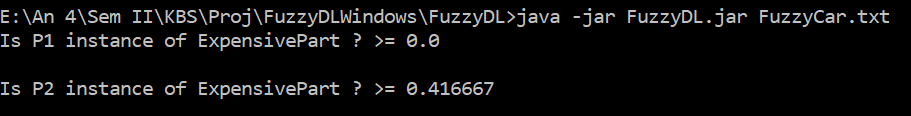
\includegraphics[width=\textwidth]{Rez.png}

\subsection{Code}
\begin{lstlisting}[language=LISP]
(define-modifier very linear-modifier(0.8))

(define-fuzzy-concept Part1PriceRange crisp(0,10000,80,1500))
(define-fuzzy-concept Part2PriceRange crisp(0,10000,6000,10000))

(define-fuzzy-concept Expensive right-shoulder(0,10000,4000,10000))

(define-concept ExpensivePart (and Part (some Price (very Expensive)))) 


(instance P1 (and Part (some Price Part1PriceRange)) 1)
(instance P2 (and Part (some Price Part2PriceRange)) 1)

(min-instance? P1 ExpensivePart)
(min-instance? P2 ExpensivePart)
\end{lstlisting}

\chapter{Queries}
\section{Racer Queries}
\begin{center}
    \pgfimage[width=17cm]{racerq.png}
\end{center}
\section{NRQL Queries}
\begin{center}
    \pgfimage[width=17cm]{nrql.png}
\end{center}
\section{Query Results}
\begin{center}
    \pgfimage[width=17cm]{racerqres.png}
\end{center}
\begin{center}
    \pgfimage[width=17cm]{nrqlres.png}
\end{center}

\chapter{Appendix}
\appendix



\section{Racer axioms}
\lstset{style=mystyle}
\begin{lstlisting}[language=Octave]
(full-reset)

; --- CONCEPTS ---
; Electric and Internal Combustion are different
(implies
    (or EV ICEV)
CarType)
(disjoint EV ICEV)

; These are Exterior options
(implies 
    (or Wheels Paint Headlights Roof) 
ExteriorOption)
(disjoint Wheels Paint Headlights Roof)

; These are Interior options
(implies 
    (or Seats Tech Trim Safety)
InteriorOption)
(disjoint Seats Tech Trim Safety)

; all are items
(implies
    (or ExteriorOption InteriorOption)
Item)

; all top categories are different
(disjoint CarType ExteriorOption InteriorOption)


; --- ATTRIBUTES ---
; Attributes of a car Model
(define-concrete-domain-attribute name :type string)

; Attributes of each part
(define-concrete-domain-attribute hasPrice :type integer)
(define-concrete-domain-attribute isOptional :type integer)

; --- ROLES ---
(define-primitive-role isCompatibleCarItem :domain CarType :range Item)
(define-primitive-role isCompatibleItemItem :domain Item :range Item :symmetric t)
(define-primitive-role isIncluded :domain Item :range Item :asymmetric t)


; --- RULES ---
; Is a car is compatibile with an item that includes another item,
; the car is also compatible withe the second item
(define-rule (?car ?item2 isCompatibleCarItem)
    (and (?car CarType) (?item1 Item) (?item2 Item) (not (same-as ?item1 ?item2))
    (?car ?item1 isCompatibleCarItem) (?item2 ?item1 isIncluded)) 
)

; Is an item includes another item, that in turn includes another item,
; the first and last items are compatible
(define-rule (?item1 ?item3 isIncluded)
    (and (?item1 Item) (?item2 Item) (?item3 Item) (not (same-as ?item1 ?item2)) (not (same-as ?item2 ?item3)) (not (same-as ?item1 ?item3))
    (?item1 ?item2 isIncluded) (?item2 ?item3 isIncluded))
)

; --- MODELS ---
(instance Taycan EV)
(instance Macan ICEV)

; --- WHEELS ---
(instance Wheels19 Wheels)
(instance Wheels20 Wheels)
(instance Wheels21 Wheels)

; --- PAINT ---
(instance MetallicPaint Paint)
(instance PearlescentPaint Paint)

; --- HEADLIGHTS ---
(instance LEDLights Headlights)
(instance MatrixLEDLights Headlights)

; --- ROOF ---
(instance CarbonRoof Roof)
(instance GlassRoof Roof)
(instance PanoramicRoof Roof)

; --- SEATS ---
(instance HeatedSeats Seats)
(instance HeatedSeats (equal isOptional 1))
(instance HeatedSeats (equal hasPrice 500))

(instance RegularSeats Seats)
(instance RegularSeats (equal isOptional 0))
(instance RegularSeats (equal hasPrice 0))

(instance SportSeats Seats)

; --- TECH ---
(instance ElectricBoot Tech)
(instance Camera Tech)
(instance ACC Tech)
(instance FullTechPack Tech)
(instance StarterTechPack Tech)

; --- TRIM ---
(instance MetalTrim Trim)
(instance WoodTrim Trim)
(instance RegularLeather Trim)
(instance NappaLeather Trim)

; --- SAFETY ---
(instance BlindSpotMonitor Safety)
(instance BlindSpotMonitor (equal isOptional 1))
(instance BlindSpotMonitor (equal hasPrice 300))

(instance FullSafetySystem Safety)
(instance FullSafetySystem (equal isOptional 1))
(instance FullSafetySystem (equal hasPrice 900))

(instance ParkingSensors Safety)
(instance ParkingAssistant Safety)

; --- PACKS & INCLUSIONS ---

; Seats packs
(related RegularSeats HeatedSeats isIncluded)
(related HeatedSeats SportSeats isIncluded)

; Light packs
(related LEDLights MatrixLEDLights isIncluded)

; Roof packs
(related GlassRoof PanoramicRoof isIncluded)

; Tech packs
(related ElectricBoot StarterTechPack isIncluded)
(related StarterTechPack FullTechPack isIncluded)
(related Camera FullTechPack isIncluded)
(related ACC FullTechPack isIncluded)

; Trim packs
(related MetalTrim RegularLeather isIncluded)
(related WoodTrim NappaLeather isIncluded)

; Safety Pack
(related ParkingSensors ParkingAssistant isIncluded)
(related ParkingAssistant FullSafetySystem isIncluded)
(related BlindSpotMonitor FullSafetySystem isIncluded)

; --- COMPATIBILITIES ---
; we only define model-item compatibility with the topmost item
; and infer item-item compatibility with lower items
(related Taycan SportSeats isCompatibleCarItem)
(related Taycan FullSafetySystem isCompatibleCarItem)
(related Taycan NappaLeather isCompatibleCarItem)
(related Taycan MatrixLEDLights isCompatibleCarItem)
(related Taycan FullTechPack isCompatibleCarItem)
(related Taycan PanoramicRoof isCompatibleCarItem)
(related Taycan Wheels20 isCompatibleCarItem)
(related Taycan Wheels21 isCompatibleCarItem)
(related Taycan PearlescentPaint isCompatibleCarItem)

(related Macan HeatedSeats isCompatibleCarItem)
(related Macan ParkingAssistant isCompatibleCarItem)
(related Macan RegularLeather isCompatibleCarItem)
(related Macan LEDLights isCompatibleCarItem)
(related Macan StarterTechPack isCompatibleCarItem)
(related Macan CarbonRoof isCompatibleCarItem)
(related Macan Wheels19 isCompatibleCarItem)
(related Macan Wheels20 isCompatibleCarItem)
(related Macan MetallicPaint isCompatibleCarItem)

(execute-all-rules)
(reexecute-all-rules)


\end{lstlisting}

\section{Ontology evaluation}
\lstset{style=mystyle}
\begin{lstlisting}[language=Octave]
(abox-consistent?)
(tbox-cyclic?)
(tbox-coherent?)

(realize-abox)
(classify-tbox)

(evaluate (length (all-individuals)))
(evaluate (length (all-atomic-concepts)))
(evaluate (length (all-roles)))
(evaluate (length (all-rules)))

(all-concept-assertions)
(all-role-assertions)
(all-constraints)

(describe-tbox)
(describe-abox)

(taxonomy)

(get-tbox-language)
(get-abox-language)


; large answer
(related-individuals isCompatibleCarItem)
(related-individuals isCompatibleItemItem)
(related-individuals isIncluded)
(individual-fillers Taycan isCompatibleCarItem)

; manually defined
(concept-disjoint? Wheels Tech) ; --> T
(individuals-related? ParkingSensors FullSafetySystem isIncluded)

; minilisp
(evaluate (> (retrieve-individual-told-attribute-value 'HeatedSeats 'hasPrice (current-abox))
(retrieve-individual-told-attribute-value 'RegularSeats 'hasPrice (current-abox))))

; deduced
(individuals-related? Taycan BlindSpotMonitor isCompatibleCarItem)
(individuals-related? Taycan ParkingSensors isCompatibleCarItem)
(individuals-related? BlindSpotMonitor Wheels19 isCompatibleItemItem)

(retrieve-individual-told-attribute-value 'HeatedSeats 'isOptional (current-abox))

; NRQL
(get-nrql-version)
(enable-nrql-warnings)
(defquery is-interior (?x) (or (?x Seats) (?x Safety) (?x Tech) (?x Trim)))
(defquery is-included (?x ?y) (?x ?y isIncluded))

; all interior items
(retrieve (?x) (?x is-interior))

; items included in other items
(retrieve (?x ?y) (?x ?y is-included))

; interior trim for Taycan
(defquery trim-options (?car ?trim) (and (?car CarType) (?trim Trim) (?car ?trim isCompatibleCarItem)))
(retrieve (?trim) (Taycan ?trim trim-options))

; models compatible with an item
(defquery compat-cars (?car ?item) (and (?car CarType) (?item Item) (?car ?item isCompatibleCarItem)))
(retrieve (?car) (?car SportSeats compat-cars))

(all-queries)


\end{lstlisting}

\section{FuzzyDL axioms}
\lstset{style=mystyle}
\begin{lstlisting}
(define-modifier very linear-modifier(0.8))

(define-fuzzy-concept Part1PriceRange crisp(0,10000,80,1500))
(define-fuzzy-concept Part2PriceRange crisp(0,10000,6000,10000))

(define-fuzzy-concept Expensive right-shoulder(0,10000,4000,10000))

(define-concept ExpensivePart (and Part (some Price (very Expensive)))) 


(instance P1 (and Part (some Price Part1PriceRange)) 1)
(instance P2 (and Part (some Price Part2PriceRange)) 1)

(min-instance? P1 ExpensivePart)
(min-instance? P2 ExpensivePart)
\end{lstlisting}

\section{Java Code}
\lstset{style=mystyle}
\begin{lstlisting}[language=Java]
package com.kbs.main;

import com.racersystems.jracer.RacerClient;

import java.io.BufferedReader;
import java.io.DataOutputStream;
import java.io.InputStreamReader;
import java.net.HttpURLConnection;
import java.net.URL;
import java.net.URLEncoder;
import java.nio.charset.StandardCharsets;
import java.util.HashMap;
import java.util.Map;

public class Main {

    private static String getParamsString(Map<String, String> params) {
        StringBuilder result = new StringBuilder();

        for (Map.Entry<String, String> entry : params.entrySet()) {
            result.append(URLEncoder.encode(entry.getKey(), StandardCharsets.UTF_8));
            result.append("=");
            result.append(URLEncoder.encode(entry.getValue(), StandardCharsets.UTF_8));
            result.append("&");
        }

        String resultString = result.toString();
        return resultString.length() > 0
                ? resultString.substring(0, resultString.length() - 1)
                : resultString;
    }

    public static void main(String[] args) {

        String input = "\"C:/Users/andre/Poli/KBS/Project/CarConfig/src/com/kbs/racer/CarOntology.racer\"";
        String queries = "\"C:/Users/andre/Poli/KBS/Project/CarConfig/src/com/kbs/racer/OntologyEvaluation.racer\"";

        try {
            URL url = new URL("http://example.com");
            HttpURLConnection con = (HttpURLConnection) url.openConnection();
            con.setRequestMethod("GET");

            Map<String, String> parameters = new HashMap<>();
            parameters.put("param1", "val");
            con.setDoOutput(true);
            DataOutputStream out = new DataOutputStream(con.getOutputStream());
            out.writeBytes(getParamsString(parameters));
            out.flush();
            out.close();

            int status = con.getResponseCode();
            System.out.println(status);
            if (status <= 299) {
                BufferedReader in = new BufferedReader(new InputStreamReader(con.getInputStream()));
                StringBuffer content = new StringBuffer();
                String inputLine;
                while ((inputLine = in.readLine()) != null) {
                    content.append(inputLine);
                }
                in.close();

                System.out.println(content);
            }

            con.disconnect();


        } catch (Exception e) {
            e.printStackTrace();
        }

        String ip = "127.0.0.1";
        int port = 8088;
        RacerClient racer = new RacerClient(ip, port);
        try {
            racer.openConnection();
            System.out.println(racer.sendRaw("(racer-read-file " + input + ")"));

            // obtain all individuals
            String answer = racer.sendRaw("(concept-instances *top*)");
            String[] result = answer.replaceAll("[()]", "").split(" ");

            // if their categories are disjoint, they are compatible
            for (String item1 : result) {
                for (String item2 : result) {
                    if (!item1.equals(item2) &&
                            !item1.equals("MACAN") &&
                            !item1.equals("TAYCAN") &&
                            !item2.equals("MACAN") &&
                            !item2.equals("TAYCAN")) {
                        boolean disjoint = racer.returnBoolean(racer.sendRaw("(evaluate (concept-disjoint-p (car (car (most-specific-instantiators '"
                                + item1 + " (current-abox)))) (car (car (most-specific-instantiators '"
                                + item2 + " (current-abox)))) (current-tbox)))"));
                        if (disjoint) {
                            racer.sendRaw("(related " + item1 + " " + item2 + " ISCOMPATIBLEITEMITEM)");
                        }
                    }
                }
            }

            System.out.println(racer.sendRaw("(racer-read-file " + queries + ")"));

            racer.closeConnection();

        } catch (Exception e) {
            e.printStackTrace();
        }
    }
}


\end{lstlisting}

\end{document}
